\newcommand{\templatesdir}{../../../templates}
\newcommand{\template}{template-slides-est}
\input{\templatesdir/\template/template}

\title[Árvores]{Árvores}
\subtitle{Conceitos, implementação e árvores binárias}

\setbeamercovered{invisible}

\immediate\write18{dots/compile.sh tree 0.4 > dots/tree.tex}
\immediate\write18{dots/compile.sh binaryTree 0.5 > dots/binaryTree.tex}
\immediate\write18{dots/compile.sh smallBinaryTree 0.8 > dots/smallBinaryTree.tex}
\immediate\write18{dots/compile.sh linkedBinaryTree 0.5 > dots/linkedBinaryTree.tex}

\begin{document}

\maketitle

\begin{frame}{Material de consulta}
	\textbf{Leitura obrigatória:}
	\begin{itemize}
		\item Capítulo 5 de~\cite{EdelweissAndGalante2009} -- Árvores.
	\end{itemize}
	
	\bigskip
	
	\textbf{Leitura complementar:}
	\begin{itemize}
		\item Capítulo 8 de~\cite{GoodrichEtAl2014} -- Árvores.
		\item Capítulo 14 de~\cite{Pereira2008} -- Árvores.
	\end{itemize}
\end{frame}


\begin{frame}{Conceitos básicos}
	\textbf{Árvore}
	\begin{itemize}
		\item Estrutura de dados que modela \textbf{dependência} ou \textbf{hierarquia}.
		\begin{itemize}
			\item Elementos não são organizados de maneira linear.
		\end{itemize}
	
		\item Representada graficamente por um conjunto de nodos interligados.
	\end{itemize}
	
	\bigskip
	
	\begin{figure}
		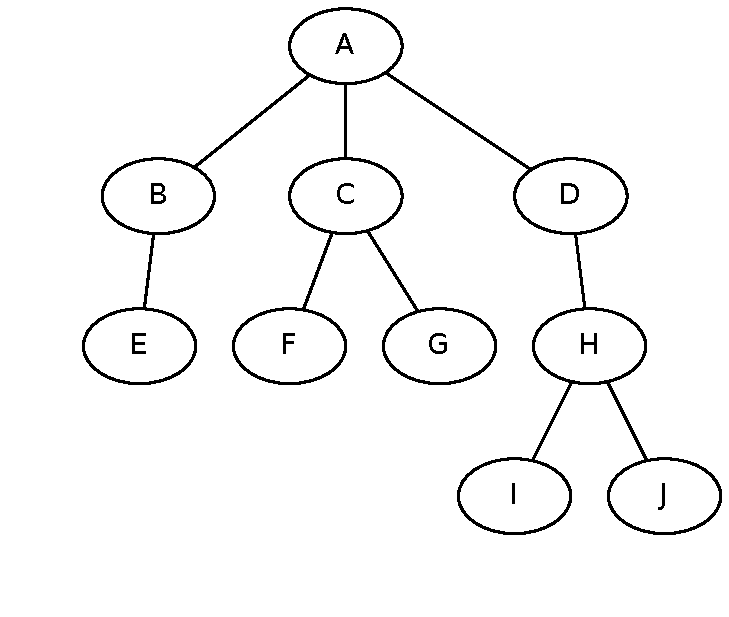
\includegraphics[width=0.4\linewidth]{dots/tree}

	\end{figure}
\end{frame}


\begin{frame}{Exemplos}
	\begin{itemize}
		\item \textbf{Hierarquias de especialização} (classes/sub-classes):
		\begin{itemize}
			\item Tipos de veículos:
			\begin{itemize}
				\item Aquático (barco, canoa).
				\item Aéreo (avião, helicóptero).
				\item Terrestre (carro, moto).
			\end{itemize}
		\end{itemize}
	
		\pause
	
		\item \textbf{Hierarquias de composição} (todo/parte):
		\begin{itemize}
			\item Um carro é composto por chassi, motor e rodas.
		\end{itemize}
	
		\pause
		
		\item \textbf{Hierarquias de subordinação ou dependência}:
		\begin{itemize}
			\item Uma empresa organiza seus cargos e setores hierarquicamente:
			\begin{itemize}
				\item Presidência comanda diretores.
				\item Diretores comandam gerentes.
				\item Gerentes comandam operadores.
			\end{itemize}
		\end{itemize}
	\end{itemize}

	\pause
	
	\begin{tikzpicture}[remember picture,overlay,shift={(current page.center)}]
	\node [rectangle, align=center, fill=blue!27!white, rounded corners=0.05cm, opacity = 0.75, text opacity = 1, text=black] at (2.8, -3.7) {%
		\footnotesize
		Faça a representação gráfica destes exemplos.%
	};
	\end{tikzpicture}
\end{frame}

\begin{frame}[t]{Terminologia}
	
	\begin{itemize}
		\only<1>{\item \textbf{Raiz:} é o primeiro nodo da árvore, ao qual todos os demais são subordinados. O acesso à árvore sempre inicia por ele.
		\begin{itemize}
			\item $A$ é a raiz da árvore.
		\end{itemize}
		}
		
		\only<2>{\item \textbf{Nodos descendentes:} aqueles que estão abaixo de um determinado nodo mais acima, apresentando alguma relação de dependência.
		\begin{itemize}
			\item Nodos mais acima são chamados ascendentes.
			\item Descendentes diretos são chamados de \textit{filhos}.
			\item Um ascendente direto é chamado de \textit{pai}.
			\item $F$ e $G$ são descendentes/filhos de $C$ (pai) e são ditos \textit{irmãos}. 
			\item $F$ e $G$ também são descendentes de $A$.
		\end{itemize}
		}
		
		\only<3>{\item \textbf{Sub-árvore:} conjunto de nodos descendentes de um mesmo nodo.
		\begin{itemize}
			\item $C$, $F$ e $G$ formam uma sub-árvore de $A$.
			\item $H$, $I$ e $J$ formam uma sub-árvore de $D$.
		\end{itemize}
		}
		
		\only<4>{\item \textbf{Grau do nodo:} número de sub-árvores que o nodo possui. Ou seja, o número de filhos de um nodo.
		\begin{itemize}
			\item O nodo $A$ possui grau $3$.
			\item O nodo $C$ possui grau $2$.
			\item O nodo $E$ possui grau $0$.
		\end{itemize}
		}
		
		\only<5>{\item \textbf{Grau da árvore:} o maior valor entre os graus dos seus nodos.
		\begin{itemize}
			\item A árvore possui grau $3$.
		\end{itemize}
		}
		
		\only<6>{\item \textbf{Folha:} nodos de grau $0$, ou seja, que não possuem filhos.
		\begin{itemize}
			\item Também chamados de nodos terminais ou externos.
			\item As folhas da árvore são $E$, $F$, $G$, $I$ e $J$.
		\end{itemize}
		}
		
		\only<7>{\item \textbf{Nodo de derivação:} nodos de grau maior que $0$, ou seja, que apresentam filhos (sub-árvores).
		\begin{itemize}
			\item Também chamados de nodos internos.
			\item Os nodos de derivação da árvore são $A$, $B$, $C$, $D$ e $H$.
		\end{itemize}
		}
		
		\only<8>{\item \textbf{Nível do nodo:} número de ligações entre o nodo e a raiz da árvore. Corresponde à profundidade do nodo na árvore. A raiz possui nível $1$, seus filhos possuem nível $2$, etc.
		\begin{itemize}
			\item Também chamado de profundidade do nodo.
			\item Os nodos $B$, $C$ e $D$ possuem nível $2$.
			\item O nodo $I$ possui nível $4$.
		\end{itemize}
		}
		
		\only<9>{\item \textbf{Caminho:} consiste em uma sequência de nodos consecutivos distintos entre dois nodos.
		\begin{itemize}
			\item $A$ -- $D$ -- $H$ -- $J$ é um caminho na árvore.
			\item O \textit{comprimento de um caminho} é o número de ligações que ele possui (número de saltos). %O comprimento pode ser calculado como o número de níveis do caminho, menos $1$ unidade.
		\end{itemize}
		}
		
		\only<10>{\item \textbf{Altura:} a \textit{altura de um nodo} é o número de nodos do maior caminho deste nodo até um dos seus descendentes-folha. A \textit{altura da árvore} é igual ao maior nível dos seus nodos.
		\begin{itemize}
			\item Todos os nodos-folha possuem altura $1$.
			\item A altura da árvore é $4$, o que indica que existe pelo menos um nodo com distância $3$ da raiz.
		\end{itemize}
		
		}
		
		\only<11>{\item \textbf{Árvore ordenada:} é uma árvore onde a ordem das suas sub-árvores é relevante para o seu contexto.
		\begin{itemize}
			\item Se a árvore for ordenada, trocar a posição das sub-árvores com raiz $B$ e $C$ resulta em uma árvore diferente.
		\end{itemize}
		}
		
		\only<12>{\item \textbf{Árvore binária:} uma árvore cujos nodos possuem no máximo grau $2$. Ou seja, um nodo possui $0$, $1$ ou $2$ filhos.
		\begin{itemize}
			\item Uma árvore $n$-ária possui grau no máximo $n$.
			\item A árvore não é binária.
		\end{itemize}
		}
	\end{itemize}

	\begin{tikzpicture}[remember picture,overlay,shift={(current page.center)}]
		\node at (0.5, -2) {%
			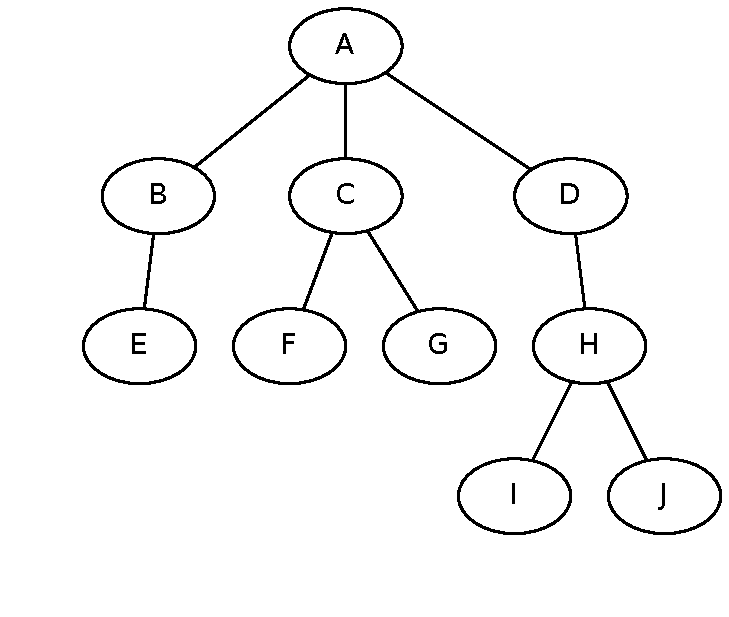
\includegraphics[width=0.4\linewidth]{dots/tree}

		};
	\end{tikzpicture}
\end{frame}

\begin{frame}{Árvores binárias}
	\begin{itemize}
		\item Seus nodos possuem no máximo dois filhos.
		\item Cada nodo possui:
		\begin{itemize}
			\item Filho da esquerda e filho da direita.
			\item Sub-árvore da esquerda e uma sub-árvore da direita.
		\end{itemize}
	\end{itemize}

	\begin{figure}
		\centering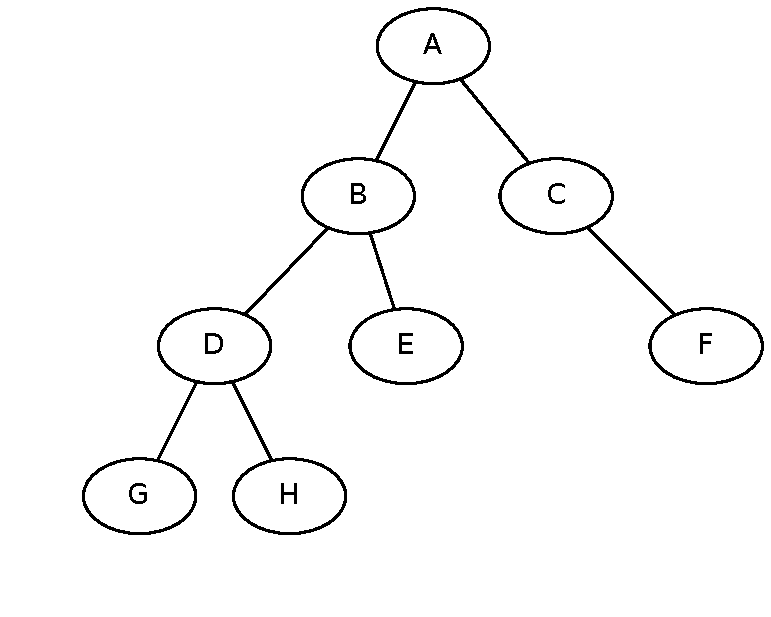
\includegraphics[width=0.5\linewidth]{dots/binaryTree}

	\end{figure}
\end{frame}

\begin{frame}{Implementação}
	\framesubtitle{Contiguidade -- vetores}
	\begin{itemize}
		\item Vetor armazena todos os nodos da árvore em uma ordem predefinida.
		\item Primeiro a raiz, depois seus filhos, depois os filhos dos seus filhos, etc.
	\end{itemize}

	\begin{columns}
		\begin{column}{0.48\textwidth}
			\begin{figure}		
				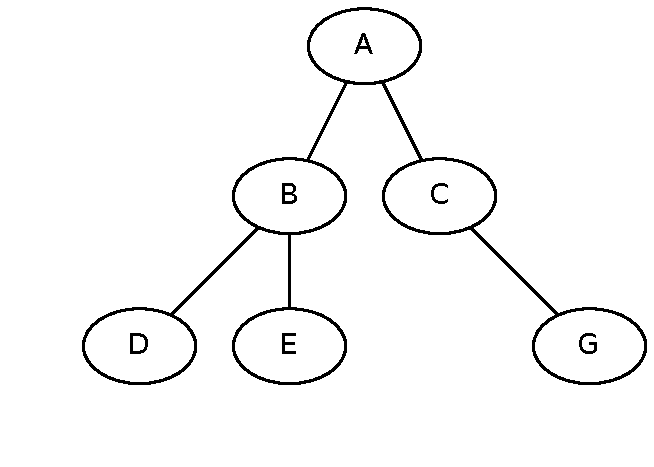
\includegraphics[width=0.8\linewidth]{dots/smallBinaryTree}

			\end{figure}
			
			\vspace{-20pt}
			
			\begin{figure}
				\scriptsize
				\begin{tikzpicture}[
					start chain = going right,
					node distance = 0pt,
					black,
					cell/.style={draw, minimum width=2em, minimum height=2em, outer sep=0pt, on chain}
				]
					\node [cell] (A) {A};
					\node [cell] (B) {B};
					\node [cell] (C) {C};
					\node [cell] (D) {D};
					\node [cell] (E) {E};
					\node [cell] (F) {\#};
					\node [cell] (G) {G};
					\node [cell] (X) {\#};
					\node [cell] (Y) {\#};
					\node [cell] (Z) {$\cdots$};
					
					\begin{scope}[-{Stealth[length = 2.5pt]}]
						\draw (A.north) [out=25, in=155] to (B.north);
						\draw (A.north) [out=30, in=155] to (C.north);
						\draw (B.south) [out=-35, in=-155] to (D.south);
						\draw (B.south) [out=-40, in=-155] to (E.south);
						\draw (C.north) [out=25, in=155] to (F.north);
						\draw (C.north) [out=25, in=155] to (G.north);
					\end{scope}
				\end{tikzpicture}
			\end{figure}
		\end{column}
		\begin{column}{0.48\textwidth}
			\pause
			\small
			\vspace{-20pt}
			\begin{block}{\small Detalhes de implementação}
				Seja um elemento $i$ da árvore:
				\begin{itemize}
					\item \texttt{leftChild}$(i) = 2i + 1$
					\item \texttt{rightChild}$(i) = 2i + 2$
					\item \texttt{parent}$(i) = \lfloor (i - 1)/2 \rfloor$
				\end{itemize}
			\end{block}
		\end{column}
	\end{columns}
\end{frame}

\begin{frame}{Implementação}
	\framesubtitle{Encadeamento}
	\begin{itemize}
		\item Cada nodo possui um apontamento para seus filhos (direita e esquerda) e para seu pai, além de armazenar o elemento correspondente.
		\item A árvore é representada através de uma referência para sua raiz.
	\end{itemize}

	\begin{figure}
		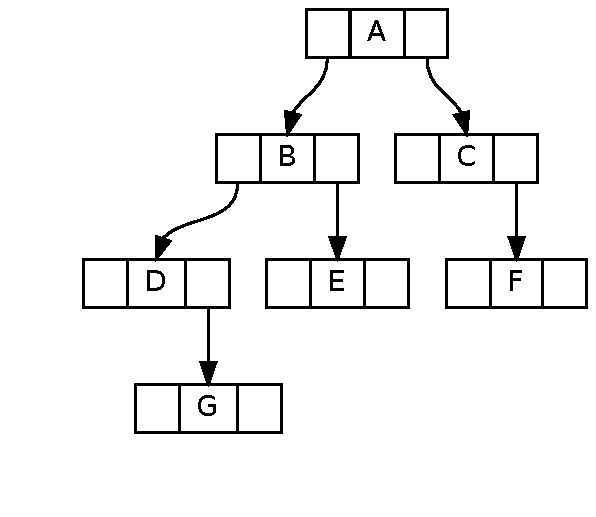
\includegraphics[width=0.5\linewidth]{dots/linkedBinaryTree}

	\end{figure}
\end{frame}

\begin{frame}{Exercício}
	\framesubtitle{Implementação com encadeamento}
	\begin{enumerate}
		\item Implemente uma árvore binária usando encadeamento. A estrutura de dados deve fornecer as seguintes operações:
		\begin{itemize}
			\item tamanho
			\item vazio
			\item inserir um elemento
			\item setar um elemento
			\item remover um elemento
			\item irmãos de um nodo
			\item profundidade de um nodo
			\item altura de um nodo
			\item verificar se um nodo é interno, externo e raiz
		\end{itemize}
	\end{enumerate}

	{\small
		\textbf{Dicas:} crie uma classe \texttt{Node} que conterá o elemento, filhos e pai; o elemento é definido pela classe \texttt{Element}; a estrutura de nodos é visível externamente.
	}

	\bigskip

	\pause
	
	\begin{tikzpicture}[remember picture,overlay,shift={(current page.center)}]
		\node [rectangle, align=center, fill=blue!27!white, rounded corners=0.05cm, opacity = 0.75, text opacity = 1, text=black] at (2.4, -4) {%
			\footnotesize
			Veja a implementação nos códigos-fonte da disciplina.%
		};
	\end{tikzpicture}
\end{frame}

\begin{frame}{Percurso}
	\begin{itemize}
		\item Um percurso (também chamado de travessia ou caminhamento) de uma árvore consiste em acessar (ou visitar) todos os seus nodos.
		\item Principais métodos de travessia de árvores:
		\begin{itemize}
			\item Pré-ordem (profundidade);
			\item Pós-ordem;
			\item In-ordem;
			\item Largura.
		\end{itemize}
		\item Esses métodos são aplicáveis a qualquer árvore.
		\item Os algoritmos percorrem toda a árvore -- complexidade $O(n)$.
	\end{itemize}
\end{frame}


\begin{frame}{Percurso em pré-ordem}
\begin{itemize}
	\item Dada uma árvore $T$, o percurso de pré-ordem:
	\begin{enumerate}
		\item visita a raiz de $T$.
		\item as sub-árvores dos filhos são visitadas recursivamente.
	\end{enumerate}
	\item Pode ser adotada alguma estratégia para explorar os filhos seguindo uma ordem desejada.
\end{itemize}

\bigskip
\bigskip

\begin{algorithm}[H]
	\DontPrintSemicolon
	Visit node $n$\;
	\ForEach{child $c$ in children(n)}{
		\texttt{preorder(c)}\;
	}

	\caption{\texttt{preorder(Node<E> n)}}
\end{algorithm}

\end{frame}


\begin{frame}{Percurso em pré-ordem}
Estratégia de profundidade:
\begin{itemize}
	\item Acessa os filhos até chegar no final da árvore.
	\item Volta e continua a busca pelos demais filhos.
\end{itemize}

\medskip

\begin{figure}
	\centering
	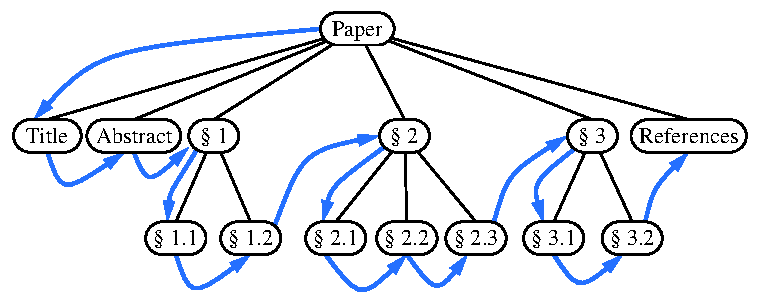
\includegraphics[width=0.75\linewidth]{img/figure-8-13}
\end{figure}
\end{frame}


\begin{frame}{Percurso em pós-ordem}
\begin{itemize}
	\item Dada uma árvore $T$, o percurso de pós-ordem:
	\begin{enumerate}
		\item visita recursivamente os filhos da raiz $T$.
		\item visita a raiz de $T$.
	\end{enumerate}
	\item Pode ser vista como o oposto da pré-ordem.
\end{itemize}

\bigskip
\bigskip

\begin{algorithm}[H]
	\DontPrintSemicolon
	\ForEach{child $c$ in children(n)}{
		\texttt{postorder(c)}\;
	}
	Visit node $n$\;
	
	\caption{\texttt{postorder(Node<E> n)}}
\end{algorithm}

\end{frame}


\begin{frame}{Percurso em pós-ordem}
Estratégia das folhas até a raiz:
\begin{itemize}
	\item Visitação começa pelas folhas.
	\item Último elemento visitado é a raiz da árvore.
\end{itemize}

\medskip

\begin{figure}
	\centering
	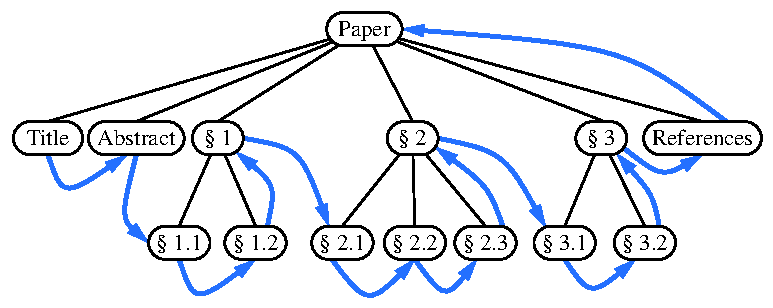
\includegraphics[width=0.75\linewidth]{img/figure-8-14}
\end{figure}
\end{frame}


\begin{frame}{Percurso em largura}
\begin{itemize}
	\item Percorre os nodos por níveis.
	\begin{enumerate}
		\item explora todos os nodos de uma profundidade.
		\item depois passa para a próxima.
	\end{enumerate}
	\item Também chamado \textit{breadth-first traversal}.
	\item Exemplo: encontrar a solução de jogos.
\end{itemize}

\medskip

\begin{figure}
	\centering
	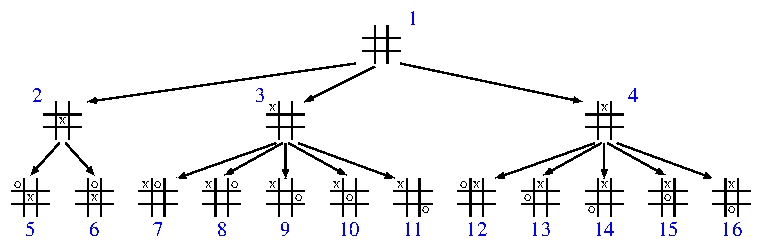
\includegraphics[width=0.85\linewidth]{img/figure-8-15}
\end{figure}
\end{frame}


\begin{frame}{Percurso em largura}
\begin{itemize}
	\item Pode-se usar uma fila para implementar a estratégia (\textit{FIFO}).
	\item Procedimento não é recursivo, pois não se aplica igualmente a sub-árvores.
\end{itemize}

\bigskip

\begin{algorithm}[H]
	\DontPrintSemicolon

	Initialize queue $Q$ to contain root\;
	\While{$Q$ is not empty}{
		$n \gets$ $Q$.dequeue()\;
		Visit node $n$\;
		\For{each child $c$ in children(n)}{
			$Q$.enqueue($n$)\;
		}
	}
	
	\caption{\texttt{breadthfirst()}}
\end{algorithm}

\end{frame}


\begin{frame}{Exercício}
	\framesubtitle{Implementação dos métodos de percurso}

	\begin{enumerate}
		\item Implemente os métodos de percurso de pré-ordem, pós-ordem e em largura na sua árvore binária usando encadeamento. Utilize esses métodos para implementar algumas tarefas:
		\begin{itemize}
			\item imprimir todos os elementos da árvore.
			\item fazer um somatório dos elementos numéricos armazenados na árvore.
			\item buscar um elemento na árvore.
		\end{itemize}
	\end{enumerate}
\end{frame}


\begin{frame}{Árvores binárias de busca}
\begin{itemize}
	\item Trata-se de uma \textbf{árvore binária ordenada}.
	\item Isso permite a busca eficiente de elementos.
	\item Propriedades:
	\begin{itemize}
		\item Nodo $n$ armazena um elemento $e(n)$.
		\item Elementos na sub-árvore \textbf{esquerda} de $n$ são \textbf{menores} que $e(n)$.
		\item Elementos na sub-árvore \textbf{direita} de $n$ são \textbf{maiores} que $e(n)$.
	\end{itemize}
\end{itemize}

\begin{figure}
	\centering
	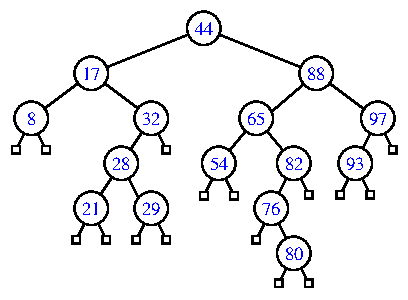
\includegraphics[width=0.55\linewidth]{img/figure-11-1}
\end{figure}
\end{frame}


\begin{frame}{Árvores binárias de busca}
\begin{itemize}
	\item Buscar um elemento em uma árvore binária de busca é similar a fazer uma busca binária (pois a árvore está ordenada).
	\begin{enumerate}
		\item Se o elemento buscado for o da raiz, retorna sucesso.
		\item Se for menor, repete a busca na sub-árvore da esquerda.
		\item Se for maior, repete a busca na sub-árvore da direita.
		\item Se chegar a alguma folha sem encontrar, elemento não existe.
	\end{enumerate}
	\item A cada iteração, metade da árvore é descartada -- complexidade $O(\log n)$.
\end{itemize}

\vspace{-5pt}

\begin{figure}
	\centering
	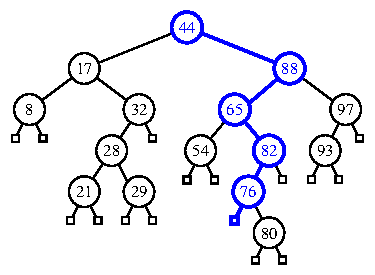
\includegraphics[width=0.55\linewidth]{img/figure-11-2b}
\end{figure}
\end{frame}



\begin{frame}{Árvores binárias de busca}
\framesubtitle{Inserção de elementos}
\begin{itemize}
	\item A inserção deve respeitar a ordem dos elementos.
	\begin{enumerate}
		\item Busca a posição correta de inserção.
		\item Insere o novo elemento.
	\end{enumerate}
	\item \textbf{Exemplo:}
	\begin{itemize}
		\item o elemento $50$ seria inserido como filho à esquerda do elemento $54$.
		\item o elemento $15$ seria inserido como filho à direita do elemento $8$.
	\end{itemize}
\end{itemize}

\begin{figure}
	\centering
	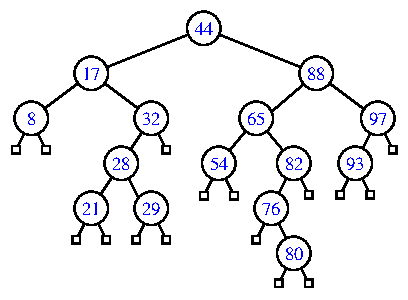
\includegraphics[width=0.55\linewidth]{img/figure-11-1}
\end{figure}
\end{frame}



\begin{frame}{Árvores binárias de busca}
\framesubtitle{Remoção de elementos}
\begin{itemize}
	\item A remoção deve manter a ordem dos elementos.
	\begin{enumerate}
		\item Remove elemento.
		\item Se nodo removido é uma folha, termina.
		\item Se nodo removido possui um filho, filho toma sua posição.
		\item Se nodo removido possui dois filhos, rearranja.
	\end{enumerate}
\end{itemize}

\begin{figure}
	\centering
	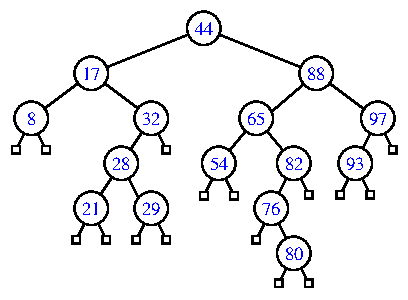
\includegraphics[width=0.55\linewidth]{img/figure-11-1}
\end{figure}

\end{frame}



\begin{frame}{Árvores binárias de busca}
\framesubtitle{Remoção de elementos}
\begin{itemize}
	\item Caso 1 -- promover filho:
	\begin{enumerate}
		\item $p$ é o elemento a remover.
		\item seu único filho $r$ toma seu lugar.
	\end{enumerate}
\end{itemize}

\begin{figure}
	\centering
	\begin{subfigure}
		\centering
		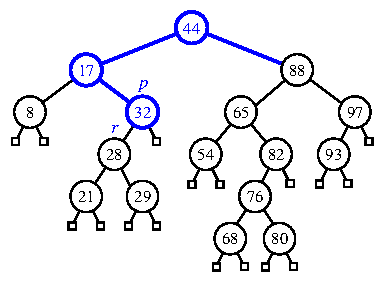
\includegraphics[width=.4\linewidth]{img/figure-11-5a}
	\end{subfigure}%
	\hspace{10pt}
	\begin{subfigure}
		\centering
		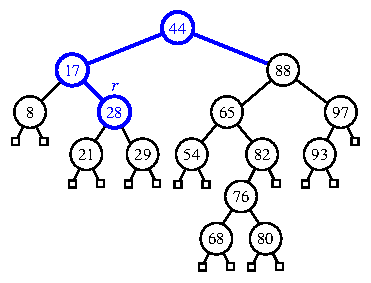
\includegraphics[width=.39\linewidth]{img/figure-11-5b}
	\end{subfigure}
\end{figure}
\end{frame}



\begin{frame}{Árvores binárias de busca}
\framesubtitle{Remoção de elementos}
\begin{itemize}
	\item Caso 2 -- rearranjar:
	\begin{enumerate}
		\item $p$ é o elemento a remover.
		\item $r$ é o maior elemento estritamente menor que $p$.
		\item $r$ toma o lugar de $p$.
		\item $r$ não terá filho à direita, portanto seu filho à esquerda toma seu lugar.
	\end{enumerate}
\end{itemize}

\begin{figure}
	\centering
	\begin{subfigure}
		\centering
		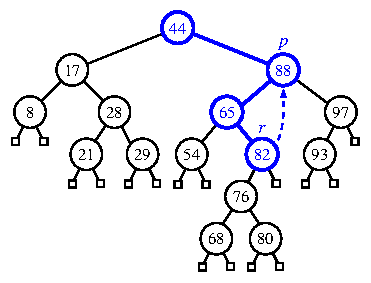
\includegraphics[width=.4\linewidth]{img/figure-11-6a}
	\end{subfigure}%
	\hspace{10pt}
	\begin{subfigure}
		\centering
		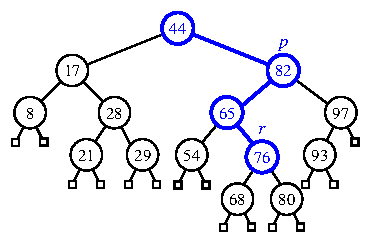
\includegraphics[width=.39\linewidth]{img/figure-11-6b}
		\begin{minipage}{.1cm}
			\vfill
		\end{minipage}
	\end{subfigure}
\end{figure}
\end{frame}



\begin{frame}{Árvores binárias de busca}
\framesubtitle{Percurso em ordem}
\begin{itemize}
	\item Aplicável a árvores binárias \textbf{ordenadas}.
	\item Dada uma árvore $T$, o percurso em ordem:
	\begin{enumerate}
		\item visita recursivamente a sub-árvore à esquerda da raiz $T$.
		\item visita a raiz de $T$.
		\item visita recursivamente a sub-árvore à direita da raiz $T$.
	\end{enumerate}
\end{itemize}

\bigskip
\bigskip

\begin{algorithm}[H]
	\DontPrintSemicolon
	\texttt{inorder(left(n))}\;
	Visit node $n$\;
	\texttt{inorder(right(n))}\;
	
	\caption{\texttt{inorder(Node<E> n)}}
\end{algorithm}
\end{frame}



\begin{frame}{Árvores binárias de busca}
\framesubtitle{Percurso em ordem}
\begin{itemize}
\item Um percurso em ordem da árvore abaixo imprimirá:
\end{itemize}

\begin{center}
	$12$ -- $25$ -- $31$ -- $36$ -- $42$ -- $58$ -- $62$ -- $75$ -- $90$
\end{center}

\begin{figure}
	\centering
	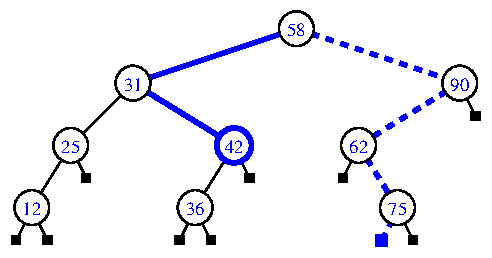
\includegraphics[width=0.6\linewidth]{img/figure-8-17}
\end{figure}
\end{frame}



\begin{frame}{Árvores binárias de busca}
\framesubtitle{Complexidade das operações}
\begin{itemize}
	\item No pior caso, uma busca vai da raiz até uma das folhas.
	\item Sendo $h$ a altura da árvore, a operação possui $O(h)$.
	\item Logo, inserção, substituição, remoção e busca em uma árvore binária de busca executam em $O(h)$.
	\item Melhor caso: $h = O(\log n)$.
	\item Pior caso: $h = O(n)$.
	\item Caso médio: $h = O(\log n)$.
	\item Variações da ABB garantem complexidade $O(\log n)$ no pior caso.
	\begin{itemize}
		\item Exemplo: arvores balanceadas.
	\end{itemize}
\end{itemize}
\end{frame}



\begin{frame}{Árvores binárias de busca}
\framesubtitle{Algumas aplicações}

\begin{itemize}
	\item Mapas:
	\begin{itemize}
		\item Armazenam elementos $\langle$chave, valor$\rangle$ de forma ordenada.
		\item Eficiente para as operações.
		\item Veja a implementação em~\cite{GoodrichEtAl2014}.
	\end{itemize}
	\bigskip
	\item Filas de prioridade:
	\begin{itemize}
		\item Armazenam elementos $\langle$chave, valor$\rangle$ onde a chave é a prioridade.
		\item Eficiente para as operações.
		\item São chamadas de \textit{heaps}.
		\item Veja a implementação em~\cite{GoodrichEtAl2014}.
	\end{itemize}
\end{itemize}
\end{frame}



\begin{frame}{Exercício}
\framesubtitle{Implementação com encadeamento}
\begin{enumerate}
	\item Implemente uma árvore binária de busca usando encadeamento. Implemente todas as operações referentes a árvores e os algoritmos de percurso estudados.
	\begin{itemize}
		\item Utilize a estrutura criada para armazenar elementos na estrutura $\langle$chave, valor$\rangle$. A chave pode ser um campo numérico, e o valor armazena objetos de uma classe qualquer.
	\end{itemize}
\end{enumerate}
\end{frame}

%\begin{frame}{Atividades}
%	
%\end{frame}

\frame{
	\frametitle{Referências}	
	\setlength{\bibsep}{8pt plus 0.3ex}
	\fontsize{10pt}{10}\selectfont
	\bibliographystyle{apalike}
	\bibliography{../referencias}
}

\end{document}